\documentclass{article}

% if you need to pass options to natbib, use, e.g.:
% \PassOptionsToPackage{numbers, compress}{natbib}
% before loading nips_2016
%
% to avoid loading the natbib package, add option nonatbib:
% \usepackage[nonatbib]{nips_2016}

\usepackage[final]{nips_style}
\usepackage[utf8]{inputenc} % allow utf-8 input
\usepackage[T1]{fontenc}    % use 8-bit T1 fonts
\usepackage{hyperref}       % hyperlinks
\usepackage{url}            % simple URL typesetting
\usepackage{booktabs}       % professional-quality tables
\usepackage{amsfonts}       % blackboard math symbols
\usepackage{nicefrac}       % compact symbols for 1/2, etc.
\usepackage{microtype}      % microtypography

\usepackage{amsmath}
\usepackage{latexsym}
\usepackage{graphicx}
\usepackage{amssymb}
\usepackage{mathtools}
\usepackage{bm}
\usepackage{listings}
\usepackage{subfig}
\usepackage{array}
\usepackage{multirow}
\usepackage{float}
\usepackage{subfig}


\usepackage{algorithm}
\usepackage[noend]{algpseudocode}

\makeatletter
\def\BState{\State\hskip-\ALG@thistlm}
\makeatother


\DeclareMathOperator*{\argmax}{\arg\max}
\DeclareMathOperator*{\argmin}{\arg\min}

\newcommand{\diag}[0]{\operatorname{diag}}
\newcommand{\vect}[1]{\mathbf{#1}}
\newcommand{\vects}[1]{\boldsymbol{#1}}
\newcommand{\matr}[1]{\mathbf{#1}}
\newcommand{\matrs}[1]{\boldsymbol{#1}}

\newcommand{\va}[0]{\vect{a}}
\newcommand{\vb}[0]{\vect{b}}
\newcommand{\vc}[0]{\vect{c}}
\newcommand{\vd}[0]{\vect{d}}
\newcommand{\ve}[0]{\vect{e}}
\newcommand{\vf}[0]{\vect{f}}
\newcommand{\vg}[0]{\vect{g}}
\newcommand{\vh}[0]{\vect{h}}
\newcommand{\vi}[0]{\vect{i}}
\newcommand{\vj}[0]{\vect{j}}
\newcommand{\vk}[0]{\vect{k}}
\newcommand{\vl}[0]{\vect{l}}
\newcommand{\vm}[0]{\vect{m}}
\newcommand{\vn}[0]{\vect{n}}
\newcommand{\vo}[0]{\vect{o}}
\newcommand{\vp}[0]{\vect{p}}
\newcommand{\vq}[0]{\vect{q}}
\newcommand{\vr}[0]{\vect{r}}
\newcommand{\vs}[0]{\vect{s}}
\newcommand{\vt}[0]{\vect{t}}
\newcommand{\vu}[0]{\vect{u}}
\newcommand{\vv}[0]{\vect{v}}
\newcommand{\vw}[0]{\vect{w}}
\newcommand{\vx}[0]{\vect{x}}
\newcommand{\vy}[0]{\vect{y}}
\newcommand{\vz}[0]{\vect{z}}
\newcommand{\valpha}[0]{\vects{\alpha}}
\newcommand{\vtheta}[0]{\vects{\theta}}
\newcommand{\veta}[0]{\vects{\eta}}
\newcommand{\vmu}[0]{\vects{\mu}}

\newcommand{\mA}[0]{\matr{A}}
\newcommand{\mB}[0]{\matr{B}}
\newcommand{\mC}[0]{\matr{C}}
\newcommand{\mD}[0]{\matr{D}}
\newcommand{\mE}[0]{\matr{E}}
\newcommand{\mF}[0]{\matr{F}}
\newcommand{\mG}[0]{\matr{G}}
\newcommand{\mH}[0]{\matr{H}}
\newcommand{\mI}[0]{\matr{I}}
\newcommand{\mJ}[0]{\matr{J}}
\newcommand{\mK}[0]{\matr{K}}
\newcommand{\mL}[0]{\matr{L}}
\newcommand{\mM}[0]{\matr{M}}
\newcommand{\mN}[0]{\matr{N}}
\newcommand{\mO}[0]{\matr{O}}
\newcommand{\mP}[0]{\matr{P}}
\newcommand{\mQ}[0]{\matr{Q}}
\newcommand{\mR}[0]{\matr{R}}
\newcommand{\mS}[0]{\matr{S}}
\newcommand{\mT}[0]{\matr{T}}
\newcommand{\mU}[0]{\matr{U}}
\newcommand{\mV}[0]{\matr{V}}
\newcommand{\mW}[0]{\matr{W}}
\newcommand{\mX}[0]{\matr{X}}
\newcommand{\mY}[0]{\matr{Y}}
\newcommand{\mZ}[0]{\matr{Z}}
\newcommand{\mSigma}[0]{\matrs{\Sigma}}

\DeclareMathOperator*{\E}{E}
\DeclareMathOperator*{\tr}{tr}
\DeclareMathOperator*{\prox}{prox}
\DeclareMathOperator*{\conv}{conv}
\DeclareMathOperator*{\minimize}{minimize}
\DeclareMathOperator*{\maximize}{maximize}
\DeclareMathOperator*{\sign}{sign}
\DeclareMathOperator*{\vecop}{vec}
\DeclareMathOperator*{\Poisson}{Poisson}
\DeclareMathOperator*{\Cat}{Cat}
\DeclareMathOperator*{\Dir}{Dir}
\DeclareMathOperator*{\Exp}{Exp}
\DeclareMathOperator*{\DiscreteUniform}{DiscreteUniform}
\newcommand{\R}{\mathbb{R}}

\DeclarePairedDelimiter{\abs}{\lvert}{\rvert}
\DeclarePairedDelimiter{\norm}{\lVert}{\rVert}
\DeclarePairedDelimiter{\inprod}{\langle}{\rangle}
\DeclarePairedDelimiter{\floor}{\lfloor}{\rfloor}

\newcommand{\AND}{\wedge}
\newcommand{\OR}{\vee}

\lstset{frame=tb,
  aboveskip=3mm,
  belowskip=3mm,
  showstringspaces=false,
  columns=flexible,
  basicstyle={\small\ttfamily},
  numbers=none,
  breaklines=true,
  breakatwhitespace=true,
  tabsize=4
}

\allowdisplaybreaks

\renewcommand{\thesubsection}{\thesection \,\,(\alph{subsection})}
\renewcommand{\thesubsubsection}{\thesection \,\,(\alph{subsection})\,\,[\roman{subsubsection}]
                                 \quad Solution}

\bibliographystyle{abbrvnat}

\title{GPU Project: SGD implementation on GPUS}

\author{
  Prithvi Krishna Gattamaneni\\
  \textbf{Adithya Parthasarathy}\\
  \texttt{pkg238@nyu.edu} \\
  \texttt{ap4608@nyu.edu}
}
%xxxxxxxxxxxxxxxxxxxxxxxxxxxxxxxxxxxxxxxxxxxxxxxxxxxxxxxxxxxxxxxxxxxxxxxxxxxxxx%

\begin{document}

\maketitle

\section{Gradient descent intro} %%1
Gradient descent intro\\
The structure of several machine learning algorithms is to have a data matrix of dimensions n*d and a vector y of size n, where n is the number of data points, and d is the dimensionality. Y is a vector of predictions for each data point. This setting fits a wide range of tasks such as regression and classification. 


In each of these settings it is common to have a loss function $L(H;X,y)$. This function usually returns a scalar greater than zero, that is indicative of how well the hypothesis $H$ is able to map the data $X$ to $y$. The smaller the loss function is, the better it is able to model the data. For very trivial formulations of the loss function, it is possible to find $H$ that minimizes $L$ in closed form, but in most cases this is not true. 


In cases where no closed form exists, it is very preferable to pick a $L$ that is differentiable. Gradient descent is a technique that allows us to use this property to minimize $L(H;X,y)$ wrt $H$. The idea here is to find the differential of $L(H;X,y)$ wrt $H$ which we denote as $\nabla_{H}(L(H;X,y))$.

After initializing H, an update is made to H by the following
$$H \leftarrow H - \eta \nabla_{H}(L(H;X,y))$$
where $\eta$ is some step size (some small value, typically 0.3). By doing the above repeatedly, H eventually converges to the solution.

\section{Why SGD} %%2
The drawback of the above solution is that calculation of $\nabla_{H}(L(H;X,y))$ requires us to look at all the datapoints of $X$. This obviously does not scale very well for large datasets, as we have to visit each datapoint for every step that is taken towards optimizing $H$. In order to workaround this another approach is to take a subset of X for the calculation of $\nabla_{H}(L(H;X,y))$ at each step. In order to truly represent the distribution it is common practice to take a much smaller and random subset of size say 32, during the calculation of $\nabla_{H}(L(H;X,y))$. This is called minibatch gradient descent. However when this subset size is decreased to one, we call this stochastic gradient descent. In every epoch, all the datapoints are visited in some random order. The advantage of SGD is that even though the differential we compute at each step is not completely accurate, it represents the correct direction of the step that H needs to take while consuming far less computing power, as a result of which SGD is known to converge much faster than traditional gradient descent, and minibatch descent.
\\
A summary of the SGD approach is as follows.\\

\begin{algorithm}
	\caption{SGD}\label{sgd}
	\begin{algorithmic}[1]
		\Procedure{SGD}{}
		\State $\text{initialize H}$
		\For{i=1 to T} 
		\For{each datapoint $X_j, y_j$}
		\State {$H \leftarrow H - \eta \nabla_{H}(L(H;X_j,y_j))$}
		\EndFor
		\EndFor
		
		
		\EndProcedure
	\end{algorithmic}
\end{algorithm}


\newpage

\section{Scope for parallelism} %3
Looking at the implementation of SGD, we straight away see two embedded for loops, which is an indication of  SIMD parallelism. However it is clear that we can leverage this only if the hypothesis $H$ can be averaged out across multiple threads. In many machine learning settings this is indeed the case. The idea here is to use multiple threads, say N threads, and to have each thread then perform SGD independently of each other, and to do so on a subset of the total Dataset, that has been divided randomly amongst the N threads. After a fixed number of iterations, the idea is then to take an average of each $H_i$ for all the threads from i=1 to N. 

\section{Explanation of first implementation}
For the first attempt we assume a regression setting. The data is generated randomly using a python script and noise is added to the predictions to simulate a real dataset. We chose this approach as it easier to test our implementations with datasets of different sizes. we pick random solution vector w, which is then used to generate the solution y. The data matrix x and y is then given to the implementation.
\\\\
The approach here is to divide the dataset amongst the threads. Each thread then performs SGD on it's dataset, and after a certain number of iterations, we take the average of each threads solution to get the final result.
Formally this can be expressed as shown below.
\begin{algorithm}
	\caption{Parallel SGD with samples $X= x_0 ... x_m$, iterations T, step size $\eta$, number of threads $n$, and states $w$ }\label{psgd}
	\begin{algorithmic}[1]
		\Require $H = \frac{m}{n}, \epsilon > 0, n > 1$
		\Procedure{Parallel SGD }{}
		\State $\text{Partition X giving H samples to each thread}$
		\For{i=1 to n in parallel do } 
		\State initialise $w^i = 0$
		\For{ all t=0...T}
		\State {pick a datapoint ($X_j, y_j$)}
		\State {$w^i \leftarrow w^i - \eta \nabla_{w^i}(L(w^i;X_j,y_j))$}
		\EndFor
		\EndFor
		\EndProcedure
	\end{algorithmic}
\end{algorithm}

The code for this implementation was implemented in both main.cu and in seq.cpp, i.e a gpu and a cpu implementation of the same parallel algorithm. We now compare the performance of both the GPU and the parallel CPU implementations.


\section{Experiments}

We evaluate our methods for speed, scalability and convergence speeds on synthetic dataset created for testing purposes.

\subsection{Cluster Setup}

The experiments were conducted on a Linux machine, equipped with a Intel Xeon E5-2660 processor and a nVidia Titan Z GPU. We use 16 processors for our CPU experiments, while we vary the threads used for the GPU experiments based on the problem size.

\subsection{Data}

We generated a synthetic random dataset using Scikit learn`s libraries. We varied the variance of the distribution to create multiple datasets to test the convergence of our implementation.

\subsection{Results}

We evaluate the scaling properties of our algorithm in a series of experiments on our synthetic dataset. We test scenarios where we keep the dataset size constant and vary the number of iterations, and while keeping the iterations constant and varying the problem size. Independent of the number of iterations or the configuration, our GPU implementation was always the faster algorithm, once the memory overhead is overcome.

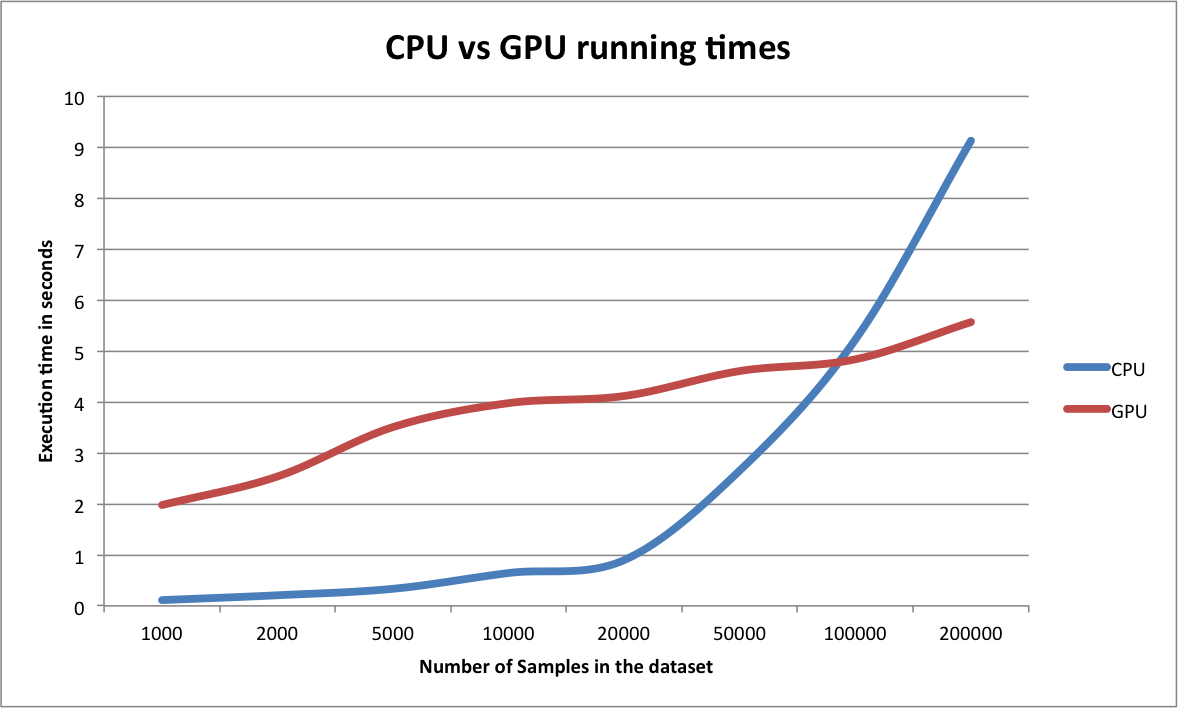
\includegraphics[scale=0.75]{cpuvgpu.png}


\subsection{Nvprof}

We used nvprof to profile our algorithm for GPU usage and time spent on different API calls. We first analyzed the point at which the GPU utilization is sufficiently large that it outweighs the memory transfer times. The results show that at a fairly small problem size, of a 40 x 5 matrix, the GPU utilization reaches a 99.2 \%. Hence, we could conclude that this problem is sufficiently large to overcome the memory overhead. Our results below illustrate the GPU usage vs iterations for a 10000 x 20 matrix.

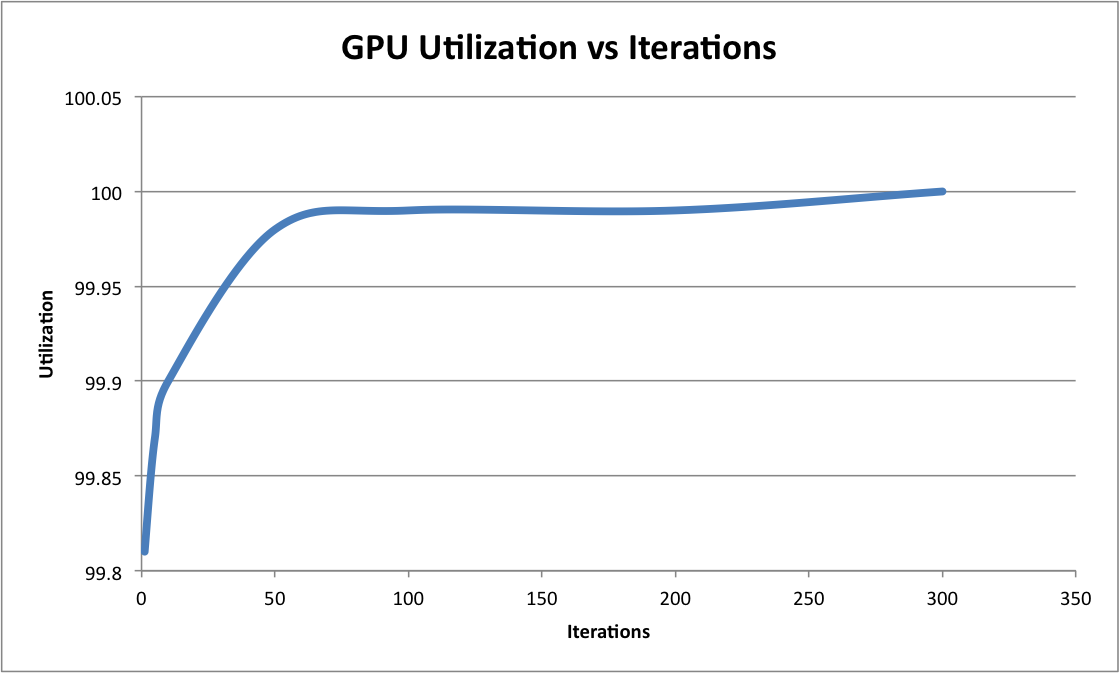
\includegraphics[scale=0.75]{utilization.png}

\pagebreak

\section{SGD with faster convergence}

While SGD parallelizes the computation the gradient of a single datapoint in a thread, the threads themselves are not sharing any information that could lead to a better convergence for the problem. One approach to improve convergence is to sync the threads once every $k$ batches and average out the weights. However, this method requires a barrier synchronization, which leads to a performance hit. The alternative approach to achieve a similar result is to use some form of asynchronous communication to speed up the convergence. We implement the ASGD algorithm proposed by Keuper and Pfreundt \textbf{cite}.

The ASGD algorithm, at every batch, compares the weights of the same batch in another thread. If they are off by a large margin, there is no update done to the weights. Otherwise, the weights are updated in a similar manner. Our results show that, when the underlying distribution has a large variation that the SGD algorithm doesn't converge well to, the ASGD algorithm provides better results with comparable execution times. We use the root mean square metric to evaluate convergence between the two methods.

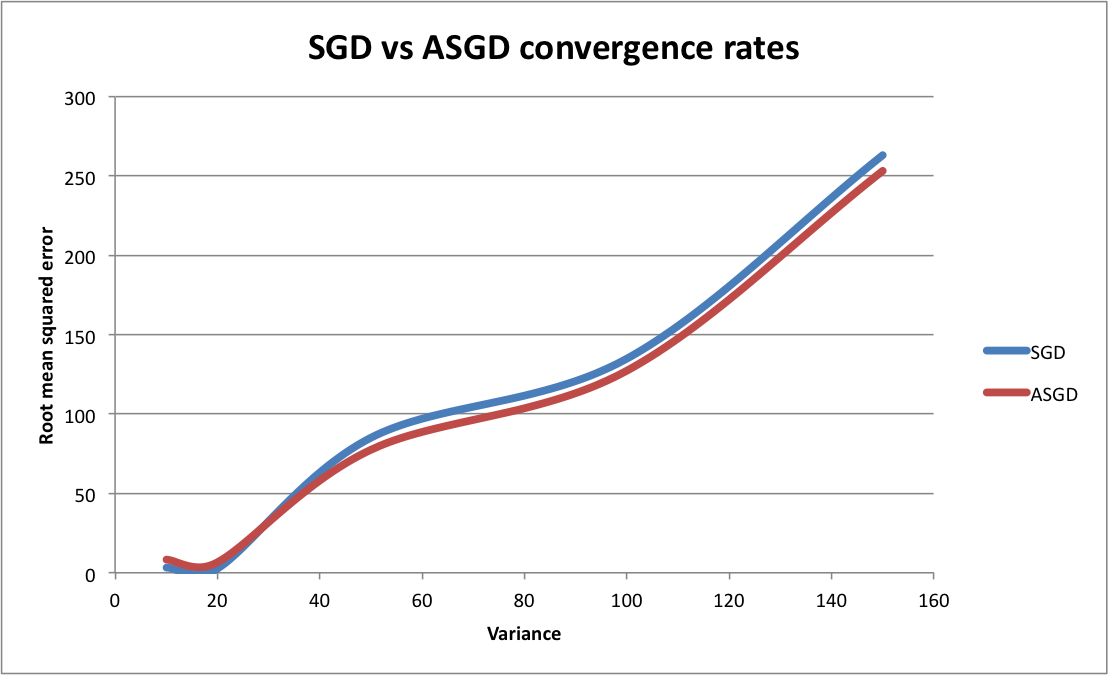
\includegraphics[scale=0.75]{sgdvasgd.png}


\end{document}
